\index{general}{Lyapunov Time}
\begin{flushright} {\tiny {\color{gray} lyapunov.tex}} \end{flushright}

Many approaches are taken in the literature when it comes 
to studying mixing/stirring in fluids, and in our case the mantle.

For example, \textcite{sato12} (2012) 
measure the convective stirring efficiency using two Lagrangian methods: 
the first determines the mixing time associated with
different wavelengths of heterogeneity following the approach of \textcite{feri01} (2001)
The second determines the value of
the maximum Finite Time Lyapunov Exponents (FTLE) as described in 
\textcite{fasa03} (2003), and measures the rate at
which heterogeneities are stretched by mantle motions.

In \textcite{taxi02} (2002) we read: 

\begin{displayquote}
{\color{darkgray}
``
Two-dimensional simulations of simple mantle convection (\textcite{chri89}, 1989; 
\textcite{ketu90}, 1990; \textcite{scha94}) suggest that for whole-mantle 
convection the mantle should be homogenized in a time-scale of less than 1 Gyr, although
unmixed islands may remain. Non-Newtonian rheology, which is thought to be 
important in the upper mantle \cite{kawu93}, may somewhat inhibit mixing (\textcite{tepy98}, 1998). 
The rate at which blobs of anomalous (e.g. primitive) material are stretched
and assimilated into the flow depends on their relative viscosity; very viscous blobs
can survive intact for many mantle overturns (\textcite{mang96}, 1996).
\\
In three-dimensional geometry with only poloidal flow, mixing may be significantly
less efficient than in two dimensions (\textcite{schh95}, 1995; \textcite{schh96}, 1996) 
but, if the toroidal flow associated with plate motions is 
included (\textcite{gaot91}, 1991), mixing can instead be more efficient 
(\textcite{feri98} (1998)).
\\
High viscosity in the deep mantle is not sufficient to maintain different reservoirs
over geological time-scales (\textcite{feri01}, 2001; van Keken \& Ballentine 1998,
1999), in contrast to predictions from earlier calculations at lower convective vigour
(\textcite{guda86b}, 1986). Part of the reason for this apparent discrepancy is that
the latter study used a kinematically driven flow rather than buoyancy-driven flow.
Since a viscosity jump does not affect densities, thermal buoyancy-driven flow has no
problem crossing it, so substantial mass exchange occurs between upper and lower
mantles. Buoyancy is thus necessary to maintain separate reservoirs.
''
}
\end{displayquote}


In \textcite{gowh06} (2006) we find
\begin{displayquote}
{\color{darkgray}
``
Heterogeneities in a convecting fluid are deformed by
stirring and finally erased by diffusive mixing. Chemical diffusion in mantle rock
acts on the scale of centimetres over the lifetime of the Earth, but our models
resolve km-scales. Therefore this paper deals only with convective stirring. Some
nice studies about mantle stirring and mixing in 2-d have been done (e.g. 
\cite{chri89,guda86b,kest91,ketu90,mebo95,olyb84,olyb84b,teyl96,teyp97,tepy98}).
Unfortunately, results from studies in 2-d can be extrapolated to 3-d only in a limited
manner. Tracers in 3-d poloidal stationary convection move on 2-d toruslike
surfaces. Stirring is constrained to these surfaces. Cross-cell stirring becomes possible
in time-dependent flows, but may not be very efficient \cite{schh96}. Large-scale stirring is
enhanced by a toroidal component, but convectively isolated islands of laminar
stirring may remain \cite{feri98}. Convection in the Earth is time-dependent and the surface
planform shows a strong toroidal component today. Since there is currently no
general understanding about the stirring behaviour of the mantle, a case-by-case
study of different models is necessary.
''
}
\end{displayquote}




%---------------------------------
\subsection{The Lyapunov exponent}

%from wiki

Simply put, the Lyapunov time is the characteristic timescale on which a dynamical system is chaotic.
 It is defined as the inverse of a system's largest Lyapunov exponent.

The Lyapunov time mirrors the limits of the predictability of the system. By convention, it is defined 
as the time for the distance between nearby trajectories of the system to increase by a factor of $e$. 
However, measures in terms of 2-foldings and 10-foldings are sometimes found, since they correspond to 
the loss of one bit of information or one digit of precision respectively.

The Lyapunov exponent or Lyapunov characteristic exponent of a dynamical system is a quantity 
that characterizes the rate of separation of infinitesimally close trajectories. 
Quantitatively, two trajectories in phase space with initial separation $\delta \mathbf{Z}_0$ 
diverge (provided that the divergence can be treated within the linearized approximation) at a rate given by
\[
|\delta \mathbf{Z} (t)|\approx e^{\lambda t}|\delta \mathbf {Z} _{0}| 
\]
where $\lambda$ is the Lyapunov exponent. 

Measuring the Lyapunov exponent or time (or related quantities) is relevant in the context of mantle stirring. 
On the one hand it is argued that the mantle is convecting and very efficient at mixing resulting in a 
somewhat homogenous composition. On the other hand, there is are modeling studies that suggest that
whole-mantle convection can preserve heterogeneity in the presence of well-mixed mantle. 

%from vazh99
Mixing takes place by the repeated stretching
and folding of interfaces. A measure of the
mixing efficiency is the time evolution of the area of
the mixing surface. Maximum efficiency of mixing
is reached with turbulent mixing behavior where
One can formally show whether mixing is laminar or turbulent by evaluating the Luyaponov exponents $\sigma$ .
These are of the form:
\[
\sigma = \lim_{t\rightarrow \infty} \lim_{X\rightarrow 0} \left[  \frac{1}{t} \ln \left( \frac{X(t)}{X(t=0)} \right)   \right]
\]
where $X(t)$ is the length of this segment at time t.
Non-zero Luyaponov exponents indicate that
stretching is exponential and the larger the exponent,
the more efficient mixing is.
However, the limits in the above equation are difficult to evaluate and the interpretation 
of the 'finite-time' Luyaponov exponent, where both limits are truncated, is difficult to formalize.


In \textcite{vazh99} (1999) the authors use a steady state velocity
pattern obtained for a model of present-day mantle convection. The velocity model is
based on the solution of the Stokes equations in a 3D spherical model with variable rheology.
To study mixing, they release particles in the velocity model and follow 
these by numerical integration. 

\begin{center}
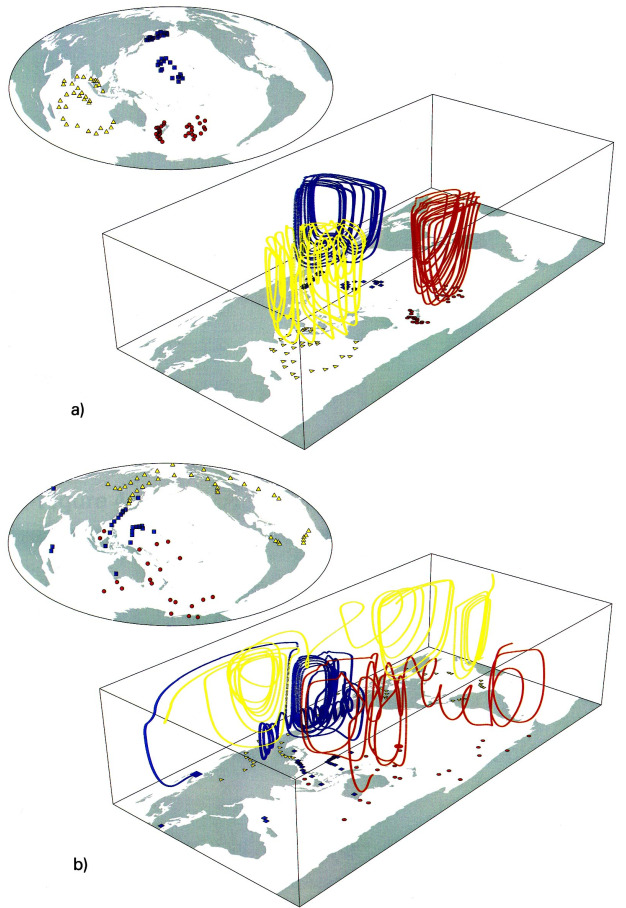
\includegraphics[width=6cm]{images/mixing/vazh99}\\
{\captionfont a) The three particles in this plot were
selected for their relatively regular pattern. 
b) Three other particles that traverse a large portion of the model. These particles feel 
the strong toroidal motion and their paths form corkscrew-like patterns. 
They indicate that certain parts of the model can exhibit strong mixing. 
Taken from \textcite{vazh99} (1999).}
\end{center}

Rather than calculating the exponents explicitly, the authors 
use an approximation to the finite-time,
finite-length Lyaponov exponent by evaluating the distance between two points that are closely spaced
at time $t=0$. For this they compute the advection of a
large number of 10 km long line segments that were
originally at 1500 km depth. The length of these segments is approximated by the distance between the
endpoints and the results are summarized in the following figure:

\begin{center}
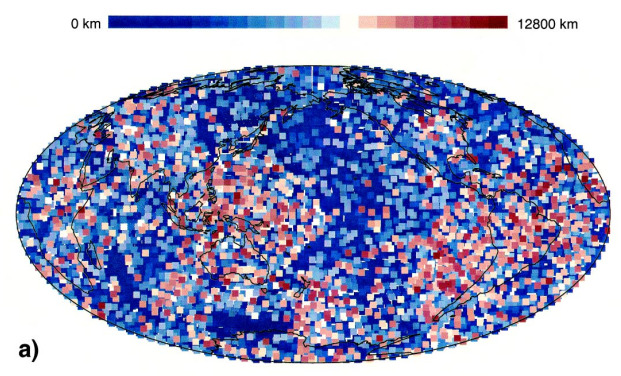
\includegraphics[width=7cm]{images/mixing/vazh99b}\\
{\captionfont Length
of the line segment after 4 billion years. Approximately 14,000 line segments were released with 
regular spacing at 1500 km depth. The length of the segment is indicated by the colored symbols 
that are plotted at the initial position. The results indicate that there is a strong
diversity in mixing behavior. In some regions (north Pacific, parts under the Indian/Australian plate) 
stretching is very limited, indicating laminar and consequently inefficient mixing. Regions that 
are under strong toroidal surface motion (western Pacific, Nazca and South
America) show very efficient stretching of up to the maximum length of the diameter of the Earth. 
Taken from \textcite{vazh99} (1999).}
\end{center}


In \textcite{becr14} (2014) the authors estimate for the first time the limit of predictability of Earth’s
mantle convection. Following the twin experiment method, we compute the Lyapunov time (i.e., e-folding
time) for state of the art 3-D spherical convection models, varying rheology, and Rayleigh number.


Reconstruction of mantle convection and surface tectonics with (ensemble) Kalman filter:
\textcite{bocf16} (2016),
\textcite{bofc18} (2018).

Investigating the initial condition
of mantle models using data assimilation. PhD thesis. \textcite{pric16} (2016).


\Literature

\textcite{pier91} (1991)
\textcite{cobs15} (2015),

%-----------------------------------------------
\subsection{configurational 'Shannon' entropy}

\textcite{gobo02} (2002), 
\textcite{cakm06} (2006),
\textcite{nake07} (2007), 
van der Wiel et al. (2024). 



%-------------------------------------------
\subsection{Literature to sort out}


\textcite{ridn82} (1982),

\textcite{gurn86} (1986),

\textcite{chri89} (1989),

\textcite{hayk92} (1992),

\textcite{scha94} (1994),

\textcite{vazh99} (1999),

\textcite{falt02} (2002),

\textcite{fasa03} (2003),

\textcite{cosc06} (2006),

\textcite{huda07b} (2007),

\textcite{mang10} (2010),

\textcite{saad11} (2011),

\textcite{vavt24} (2024)

\textcite{thsf24} (2024)


